\documentclass[11pt, a4paper]{article}

% Configuración de márgenes de las páginas
	\usepackage{a4wide}

% Paquete de acentos para Linux
	\usepackage[utf8]{inputenc}

% Paquete de acentos para windows
%	\usepackage[latin1]{inputenc}

% Paquete para reconocer la separación en sílabas en español
	\usepackage[spanish]{babel}

% Paquetes especiales para el TP
	\usepackage{./otros/caratula}
	\usepackage{./otros/algo2symb}
	\usepackage{./otros/shortlst}
	\usepackage[lined]{./otros/algorithm2e}
	\usepackage{amssymb}			%simbolos matematicos
	\usepackage{pdfpages}
	
	
% Paquete para incluir hypervinculos
	\usepackage{color}
	\usepackage{url}
	\definecolor{lnk}{rgb}{0,0,0.4}
	\usepackage[colorlinks=true,linkcolor=lnk,citecolor=blue,urlcolor=blue]{hyperref}

% Paquete para armar índices
	\usepackage{makeidx}
	\makeindex

% Más espacio entre líneas
	\parskip=1.5pt

% Comandos personalizados
	\newcommand{\nat}{\ensuremath{\mathbb{N}}}
	\newcommand{\entero}{\ensuremath{\mathbb{Z}}}
	\newcommand{\real}{\ensuremath{\mathbb{R}}}
	\newcommand{\tab}{\hspace{1em}}
	
\begin{document}

% Carátula
	\titulo{Trabajo Práctico Final}
	\fecha{Marzo de 2010}
	\materia{Organización del Computador II}
	\integrante{Bianchi, Mariano}{92/08}{marianobianchi08@gmail.com}
	\integrante{Brusco, Pablo}{527/08}{pablo.brusco@gmail.com}
	\integrante{Di Pietro, Carlos Augusto Lyon}{126/08}{cdipietro@dc.uba.ar}
	\maketitle

% Índice
\small
\newpage \printindex \tableofcontents
\normalsize
\newpage

% Cuerpo del informe
\section{Introducción}
\paragraph{}
El presente trabajo final surge como una continuación del tercer trabájo práctico de la materia en el segundo cuatrimestre de 2009. Aquél trabajo consistía en implementar un sistema minimal que permitiese correr concurrentemente dos tareas. Concretamente, dicho sistema consitía en un bootloader que se encargaba de cargar a memoria un kernel simplificado que incluía los binarios de las tareas en cuestión, junto con todas las estructuras necesarias para que dichas tareas pudieran ser ejecutadas (GDT, Directorio de Tablas de Páginas, una Tabla de Páginas para cada tarea, etc.). Luego, el kernel simplemente debía encargarse de activar el \textit{Gate A20}, pasar el procesador a modo protegido, activar el sistema de paginación, y poner a correr las tareas llamadas ``Pintor'' y ``Traductor'', las cuales alternaba mediante una interrupción del timer.

\paragraph{}
Por el contrario, el trabajo aquí presentado, si bien se basa en el anterior, posee algunas diferencias. El principal aspecto que lo diferencia es el hecho de que las tareas no se encuentran ya cargadas en memoria de manera estática, sino deben ser cargadas de manera dinámica y puestas en ejecución a través de un scheduler que va asignando tiempos de CPU a cada uno de los procesos que se ejecutan de forma concurrente en el sistema. Naturalmente, esta diferencia en cuanto al otro kernel conlleva un cambio en lo que respecta a la administracíón de memoria, ya que estructuras como entradas de la GDT o TSS's deberán ser creados e inicializados para cada nueva tarea conforme estas van siendo lanzadas.\\
En consecuencia, el resultado final es un \textit{kernel multitarea} (es decir capaz de ejecutar varias tareas alternadamente dando la ilusión de simultaneidad) que puede lanzar procesos de forma dinámica con tan solo cargar tareas de memoria y creando las estructuras necesarias para que estas puedan ejecutarse en un procesador de arquitectura Intel-x86.

		
\section{Instrucciones de uso}
\paragraph{}
Para ejecutar el kernel basta con bla bla bla.... Una vez cargado, el kernel mostrará en pantalla una consola mediante la cual se podrá cargar y poner a ejecutar cada una de las tareas. A continuación se detallan la lista de comandos que pueden ser interpretados por la consola:
\begin{itemize}
    \item "h" : ayuda (lista los comandos).
 	\item "l" : muestra todas las tareas disponibles.
 	\item "p" : muestra todas las tareas en ejecuci\'on junto con su pid.
 	\item "v \{x\}" : ejecuta y muestra la tarea \{x\}.
 	\item "d \{pid\}" : muestra la tarea con pid \{pid\}.
 	\item "k \{pid\}" : termina la tarea con pid \{pid\}.

\end{itemize}


\section{Implementación}
	\subsection{Descripción General}
	El código fuente que implementa el kernel se entrega junto con este informe en un sorpote digital y se ubica en la carpeta \texttt{codigo}. Dentro de la misma los archivos se organizan de la siguiente manera:
	\begin{center}
		\begin{shortitemize}
			\setlength{\shortitemwidth}{200pt}
			\item Memoria
			\item Scheduler
			\item GDT - Global Descriptor Table
			\item Periféricos
			\item Paginación				
			\item Consola
			\item Pantalla
			\item TSS - Task State
			\item Macros
			\item BCP - Block Control Process
			\item Almacenamiento
			\item Interrupciones							
			\item Kernel
		\end{shortitemize}
	\end{center}		

	\paragraph{}
	Esta distribución no es arbitraria, sino que responde a la modularización con la cual se encaró el diseño y desarrollo del kernel aquí presentado. Así, cada directorio contiene el código fuente uno o más de los módulos que integran al kernel, cada uno de los cuales fue desarrollado de forma incremental y testeado individualmente.
	
	\paragraph{}
	En la sección \ref{modulos}, se procederá a explicar en detalle cada uno de estos módulos a fin de poder comprender con claridad todas las partes que componen al kernel elaborado. Una vez concluída esa explicación, en la sección siguiente (\ref{kernel}), se detallará de qué forma el kernel agrupa y hace uso de todos estos módulos a fin de dar como resultado un sistema \textit{multitasking} con un \textit{scheduler} dinámico capaz de levantar tareas de memoria y alternarlas por medio de una política de reemplazo \textit{Round Robin}.
	
	\paragraph{}
	Seguidamente, se expone cómo está constituído el \textit{Mapa de memoria} del sistema, así como también el porqué de su elección.
	
	\subsection{Mapa de Memoria}
	\paragraph{}
	Previo a la escritura del código de los módulos mencionados en la sección anterior, a sabiendas de que el sistema utilizaría la paginación como forma de direccionar a memoria, se procedió a establecer un mapa de memoria que permitiese ubicar las estructuras críticas e indispensables del sistema de manera inequívoca. La opción elegida fue realizar un \textit{identity mapping} de las páginas (todas ellas de 4 KB) a los frames de memoria, fijando algunos de ellos para uso exclusivo del kernel o de otras estructuras como la \textit{GDT}, las \textit{TSS} o el \textit{Bitmap}.
	
	\paragraph{}
	La imagen que sigue muestrá como estan mapeadas y ocupadas las páginas de memoria en el sistema:
	\begin{center}
		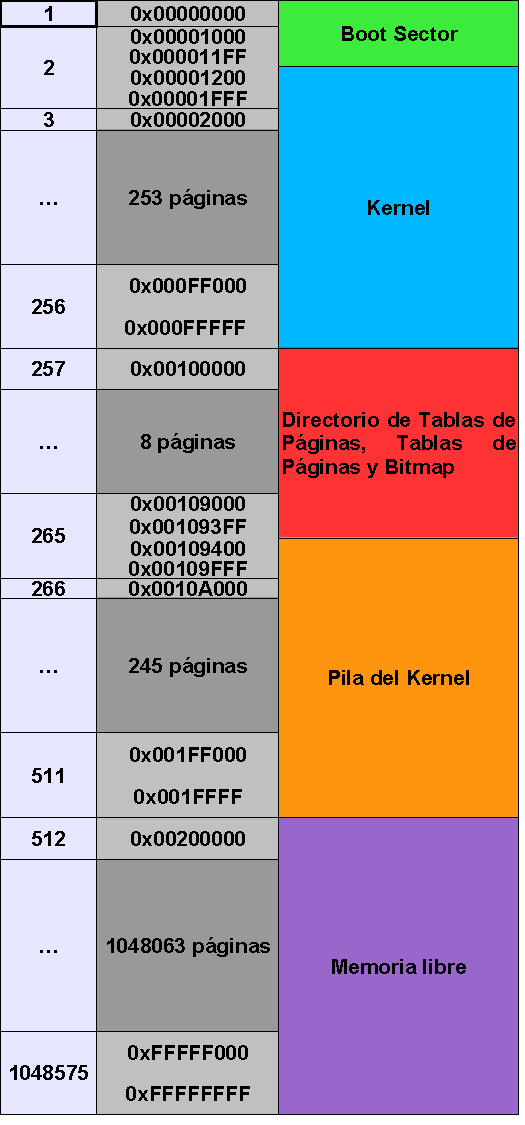
\includegraphics[scale=0.80]{./otros/mapa_memoria.pdf}
	\end{center}
	
	\subsection{Módulos}
	\label{modulos}
		\subsubsection{Memoria}
			\paragraph{}
			El módulo de \textbf{Memoria} es el encargado de brindarle al kernel las herramientas para contabilizar y administrar la memoria del sistema.
			
			\paragraph{}
			Básicamente, la idea empleada para administrar consiste en contabilizar la cantidad de bytes con los que cuenta la memoria, luego determinar cuántas páginas de 4 KB hay en la memoria del sistema y luego plasmar esta información en un \textit{Bitmap}. El \textit{Bitmap} no es más que una porción de memoria en donde hay tantos bits como páginas haya en el sistema. Luego, cada página ocupada se representa en el \textit{Bitmap} poniendo un ``1'' en el bit asociado a dicha página, mientras que las páginas libres se representan con un ``0''.
			
			\paragraph{}
			En líneas generales la interfaz de este módulo puede ser caracterizada de la siguiente manera:
			\begin{itemize}
				\item Variables Globales:
				\begin{itemize}
					\item \texttt{memoria\_total:} Variable global en la cual se almacena la cantidad de Megabytes de memoria con la que cuenta el sistema.
					\item \texttt{paginas\_libres:} Variable global que contabiliza el número de páginas libres de memoria en el sistema.
					\item \texttt{dir\_init\_bitmap:} Puntero a la dirección 0x???, que es la posición donde se inicia el \textit{Bitmap} para administrar las páginas de memoria.
					\item \texttt{dir\_end\_bitmap:} Puntero a la dirección 0x??, que es la última dirección válida del \textit{Bitmap}.
				\end{itemize}
				
				\item Funciones:
				\begin{itemize}
					\item \texttt{contarMemoria:} Función que se encarga de contar cuántos MB de memoria hay en el sistema guardando dicho valor en la variable \texttt{memoria\_total}. Asímismo, determina el número de frames de 4 KB que puede haber en la memoria del sistema y almacena dicho valor en la variable \texttt{paginas\_libres}.
					\item \texttt{llenarBitmap:} Función que a partir de la posición apuntada por \texttt{dir\_init\_bitmap} marca poniendo en ``1'' todos los bits correspondientes a las páginas de memoria utilizadas por el kernel y luego pone en ``0'' a las restantes.
					\item \texttt{pidoPagina:} Función que devuelve un puntero a la primer posición de memoria de una pagina libre, y previo a ello, la marca como ocupada en el Bitmap poniendo en ``1'' el bit correspondiente a dicha página.
					\item \texttt{liberoPagina:} Función que dado un puntero a una posicion de memoria, determina en qué página de memoria se alberga dicha posición y luego pone en ``0'' el bit correspondiente a esa página para así marcarla como libre.
					\item \texttt{setmem:} Función que dado un puntero a una posición de memoria y dos valores enteros \textit{set} y \textit{cant}, pone el valor de \textit{set} en \textit{cant} bytes desde la posición de memoria apuntada por el puntero en adelante.
					\item \texttt{cpmem:} Función que dados dos punteros a posiciones de memoria y un valor entero \textit{cant}, copia el valor de \textit{cant} bytes desde la posición de memoria apuntada por el primer puntero en adelante, hacia los \textit{cant} bytes de memoria desde la posición de memoria apuntada por el por el segundo puntero en adelante.
				\end{itemize}
			\end{itemize}

		\subsubsection{Global Descriptor Table (GDT)}
			\paragraph{}
			El módulo de \textbf{GDT} es aquel mediante el cual se introduce la estrutura de datos \textit{GDT} que modela la estructura \textit{Global Descriptor Table} de la arquitectura IA-32 de Intel\footnote{Intel 64 and IA-32 Architectures Software Developer’s Manual, Volume 3A: System Programming Guide, Part 1 - Sección 2.1.1, página 61}. Asímismo, implementa también las funcionalidades necesarias para que el kernel pueda operar y hacer uso de esta estructura.
			
			\paragraph{}
			Concretamente, la implementación de la estructura \textit{GDT} no es más que un arreglo de otra estructura más pequeña definida en este mismo módulo: la \textit{GDT\_entry}. Dicha estructura constituye un bloque de memoria de 4 bytes que modela las entradas en la \textit{GDT}, las cuales reciben el nombre de descriptores. Los descriptores pueden ser de varios tipos (descriptor de segmento, descriptor de TSS, etc) y se separan en diversos campos \footnote{Más información sobre descriptores de}. Por tal motivo, la estructura \textit{GDT\_entry} también está subdividida en idénticos campos los cuales, segun los valores que se le fijen, indican entre otras cosas a qué tipo de descriptor corresponde cada entrada.
			
			
				
		\subsubsection{Paginación}
		\subsubsection{TSS}
		\subsubsection{Process Control Block (BCP) }
		
			\paragraph{}
			El Process Control Block, es una estructructura de datos en el Kernel que contiene la información necesaria para manejar cada uno de los procesos.
			En nuestro caso, esta estructura contiene la siguiente información:
\begin{itemize}
\item \textbf{pid}: indice de la tarea en el gdt\_vector
\item \textbf{estado}: indica el estado de la tarea
\item \textbf{entrada\_directorio}: direccion del directorio de la tarea
\item \textbf{sig}: siguiente tarea para el round robin scheduler
\item \textbf{ant}: anterior tarea para el round robin scheduler
\item \textbf{pantalla}: puntero a la pagina destinada al video de la tarea
\item \textbf{nombre}
\end{itemize}

			\paragraph{}
				Ya que el BCP contiene informacion critica de los procesos, esta almacenada en un area protegida de los usuarios. En nuestro caso esta situada en !!!!!!!!!
		
			\paragraph{}
				Las principales funciones del modulo BCP son las siguientes:
				
				\begin{itemize}
	
                  
                  \item \textbf{iniciar\_BCP}: llena el BPC[0] con los datos del kernel, y inicializa variables globales

          
                  \item \textbf{buscar\_entradaBCP\_vacia }: busca entrada libre en el BCP (libre significa estado muerto)
                 
                  \item \textbf{crear\_entradaBCP }: llena la entrada con los datos de la tarea y la agrega al final de la cola de tareas activas
   
                  \item \textbf{cambiar\_estado}: cambia el estado de una tarea, y si el estado es MUERTO la quita de la cola de tareas activas
   
                  \item \textbf{buscar\_entradaBCP}: devuelve la posicion en la BCP de una tarea pasada como parametro.
     
                  \item \textbf{buscar\_entradaBCP\_matar}: devuelve la posicion en la BCP de alguna tarea con estado "MUERTA". Si no hay ninguna, devuelve CANT\_TAREAS

                  
                  \item \textbf{cargarTarea}: carga una tarea y todo sus datos y contexto en memoria y la agrega en la BCP para incluirla en el scheduling

                  
                  \item \textbf{matarTarea}: Marcar tarea como "MATAR" para que luego el KERNEL se encargue de eliminarla. 
                                   
                  \item \textbf{exit}:  esta es llamada cuando la tarea actual quiere terminar y llama a la interrupcion 80

                  
                  \item \textbf{desaparecerTarea}: Esta funcion se va a llamar cada vez que se ejecute el kernel. La idea es que si hay alguna tarea en la BCP marcada como "MATAR" (ya va a estar fuera del scheduler), esta funcion se encargue de eliminar y liberar todas las estructuras utilizadas por la tarea (BCP, TSS, directorio y tablas de páginas, paginas de video y de pila y gdt).

                  	
		
				\end{itemize}
		\subsubsection{Interrupciones}
		\subsubsection{Scheduller}
		\subsubsection{Periféricos}
		\subsubsection{Consola}
			\paragraph{}
				La consola es una función del kernel que permite una interfaz hacia los usuarios, en este caso es una linea de comandos que permite listar, correr, matar, etc. una lista de tareas disponibles en el sistema. 
			\paragraph{}
				A continuación se listan las principales funciones necesarias para hacer posibles la linea de comandos:
				\begin{itemize}

                    \item \textbf{ cargar\_tarea}: recibe la posicion de la tarea a cargar dentro de "tareas\_en\_memoria"

                    \item \textbf{console}: Es la función llamada cada vez que se preciona una tecla en la linea de comandos. En caso que esta tecla sea un 'enter' se llama a la función 'run' del comando almacenado, en caso contrario se van almacenando las teclas.
                    \item \textbf{run}: Es la encargada de obtener y decodificar el comando enviado por console de manera de llamar a la función correcta.
			
				
				
				\end{itemize}				
	


		
     	\subsubsection{Pantalla}
		\subsubsection{Macros}
		\subsubsection{Almacenamiento}
	\subsection{Ensamblando el Kernel}
	\label{kernel}	
		\begin{itemize}
			\item Habilitar Gate A20
			\item Inicializar la GDT y el GDT\_desc
			\item Copiar GDT\_desc a lgdt
			\item Habilitar bit PE de CR0
			\item Jmp 0x08:modo\_protegido
			\item Pasaje a modo protegido
			\item Actualizar selectores
			\item Inicializar la pila
			\item Contar memoria disponible
			\item Crear estructuras de paginación
			\item Cargar en CR3 la direccion del Directorio de Tablas de Páginas
			\item Habilitar bit PG de CR0
			\item Inicializar Bitmap
			\item Pasaje a paginación
		\end{itemize}
	
\end{document}
